\documentclass[a4paper]{article}

\usepackage{fullpage} % Package to use full page
\usepackage{parskip} % Package to tweak paragraph skipping
\usepackage{tikz} % Package for drawing
\usepackage{amsmath}
\usepackage{hyperref}
\usepackage{amssymb}
\usepackage{tikz-qtree}

%https://tex.stackexchange.com/questions/229355/algorithm-algorithmic-algorithmicx-algorithm2e-algpseudocode-confused
\usepackage{algorithm}
\usepackage{algorithmicx}
\usepackage{algpseudocode}

\usepackage{graphicx}
\graphicspath{ {./resources/} }

%https://tex.stackexchange.com/questions/165021/fixing-the-location-of-the-appearance-in-algorithmicx-environment
\usepackage{float}% http://ctan.org/pkg/float

%https://tex.stackexchange.com/questions/25369/how-to-rotate-a-table
\usepackage[graphicx]{realboxes}
\title{Dynamic Programming}

\begin{document}
\maketitle

Dynamic programming, like the divide-and-conquer method, solves problems by combining the solutions to \textcolor{red}{sub-problems}. (``Programming" in this context refers to a \colorbox{red}{tabular} method.)\\
\begin{itemize}
    \item \textbf{Divide-and-conquer}\\
    Partition the problem into disjoint sub-problems.\\
    Solve the sub-problems recursively.\\
    Solve the common sub-problems repeatedly.\\
    Combine their solutions.
    \item \textbf{Dynamic Programming}\\
    Sub-problems share sub-sub-problems.\\
    Solve each sub-sub-problem just once and then saves its answer in a table.
\end{itemize}
Dynamic programming is to find \textit{an} optimal solution, as opposed \textit{the} optimal solution, since there may be several solutions that achieve the optimal value. 
\\
\\
The sequence of four steps to follow:
\begin{enumerate}
    \item Characterize the structure of an optimal solution.
    \item Recursively define the value of an optimal solution.
    \item Computer the value of an optimal solution, typically in a bottom-up fashion.
    \item Construct an optimal solution from computed information.
\end{enumerate}

\section*{15.1 Rod cutting}
Given a rod of length $n$ inches and an array of prices that contains prices of all pieces of size smaller than $n$. Determine the maximum value obtainable by cutting up the rod and selling the pieces.\\
Note that we can cut a rod of length $n$ in $2^{n-1}$ ways, since we have an independent option of cutting, or not cutting, at distance $i$ inches from the left end, for $i=1,2,\ldots, n-1$.\\ 
For example, we can choose not cut at $1^{st}$ and cut at $2^{nd}$ inch, then we have a 2 inches rob.
$$
r_n=max(p_n, r_1+r_{n-1}, r_2+r_{n-2},\cdots, r_{n-1}+r_{1})
$$
The rot-cutting problem exhibits \textbf{\textit{optimal substructure}}: optimal solutions to a problem incorporate optimal solutions to related sub-problems.\\
\\
Think it in a different way:
    $$r_n=\max_{1\leq i\leq n}(p_i+r_{n-1})$$
    
\subsection*{Recursive top-down implementation}
\begin{algorithm}[H]% Use "stay right HERE" already!
    \caption{CUT-ROD($p,n$)}
    \begin{algorithmic}[1] % The number tells where the line numbering should start
        \If{$n==0$}
            \State \textbf{return }$0$
        \EndIf
        \State $q=-\infty$
        \For{$i=1$ \textbf{to} $n$}
        \State $q=max(q,p[i]+\text{CUT-ROD}(p,n-i))$
        \EndFor
    \end{algorithmic}
\end{algorithm}
Why is CUT-ROD inefficient? (Calling itself recursively)

\subsection*{Using dynamic programming for optimal rod cutting}
Solve the same sub-problems repeatedly $\Rightarrow$ Solve each sub-problem only \textit{once}.\\
So it uses additional memory to save sub-problem: \textbf{\textit{time-memory trade-off}}\\
\\
Two equivalent ways to implement a dynamic programming approach:
\begin{enumerate}
    \item top-down with memoization
    \item bottom-up method
    \begin{algorithm}[H]% Use "stay right HERE" already!
    \caption{BOTTOM-UP-CUT-ROD($p,n$)}
    \begin{algorithmic}[1] % The number tells where the line numbering should start
        \State let $r[0\ldots n]$ be a new array
        \State $r[0]=0$
        \For{$j=1$ \textbf{to} $n$}
            \State $q=-\infty$
            \For{$i=1$ \textbf{to} $j$}
            \State $q=max(q,p[i]+r[j-i])$
            \EndFor
            \State $r[j]=q$
        \EndFor
        \State \textbf{return} $r[n]$
    \end{algorithmic}
\end{algorithm}
\end{enumerate}

\subsection*{Reconstructing a solution}
skip
\subsection*{Example}
Given a rod of length n inches and an array of prices that contains prices of all pieces of size smaller than n. Determine the maximum value obtainable by cutting up the rod and selling the pieces. Assume total 5 inches, and
    $$
    \begin{array}{c|cccc}
    length & 1 & 2 & 3 & 4\\
    \hline
    price & 2 & 5 & 7 & 8
    \end{array}
    $$
    
    $$
    \begin{array}{c|cccccc}
    (price)length(i)/total(j)& 0 & 1 & 2 & 3 & 4 & 5\\
    \hline
    (2)1 & 0 & 2 & 4 & 6 & 8 & 10 \\
    (5)2 & 0 & 2 & 5 & 5+2=7 & 5+5=10 & 5+7=12 \\
    (7)3 & 0 & 2 & 5 & 7 & 10 & 7+5=12 \\
    (8)4 & 0 & 2 & 5 & 7 & 10 & 12
    \end{array}
    $$
    $$
    T[i][j]=
        \begin{cases}
        max(T[i-1][j], Price[i]+ T[i][j-i]),  & \text{if $j \geq i$} \\
        T[i-1][j], & \text{else}
        \end{cases}
    $$
    
\section*{15.2 Matrix-chain multiplication}
$$A_{p\times q} B_{q\times r}\Rightarrow C=AB \text{ needs } pqr \text{ times multiplications.}$$

\subsection*{Applying dynamic programming}
\begin{enumerate}
    \item The structure of an optimal parenthesization.\\
    Suppose that to optimally parenthesize $A_iA_{i+1}\cdots A_j$, we split the product between $A_k$ and $A_{k+1}$. Then the way we parenthesize the ``prefix" subchain $A_iA_{i+1}\cdots A_k$ within this optimal parenthesization of $A_iA_{i+1}\cdots A_j$ must be an optimal parenthesization of $A_iA_{i+1}\cdots A_k$.
    \item Recursively define the value of an optimal solution.\\
    Let $m[i,j]$ be the minimum number of scalar multiplications needed to compute the matrix $A_{i.. j}$
    $$
    m[i,j]=m[i,k]+m[k+1,j] +p_{i-1}p_kp_j
    $$
    So we only need to check the value of $k$ from $i$ to $j-1$
    $$
    m[i][j]=
        \begin{cases}
        0, & \text{if } i=j\\
        \min_{i\leq k <j}\{m[i,k]+m[k+1,j] +p_{i-1}p_kp_j\},  & \text{if $i<j$}
        \end{cases}
    $$
    Let $s[i,j]$ be a value of $k$ at which we split the product $A_iA_{i+1}\ldots A_j$ in an optimal parenthesization.
    \item Computer the value of an optimal solution, typically in a bottom-up fashion.\\
    Instead of computing the solution recursively, we compute the optimal cost by using a tabular, bottom-up approach.
    \begin{enumerate}
        \item a sequence $p=\langle p_1,p_2,\ldots, ,p_n\rangle $
        \item table $m[1..n, 1..n]$ for storing the $m[i,j]$ costs
        \item table $s[1..n-1,2..n]$ for recording which index of $k$ achieved the optimal cost in computing $m[i,j]$
    \end{enumerate}
    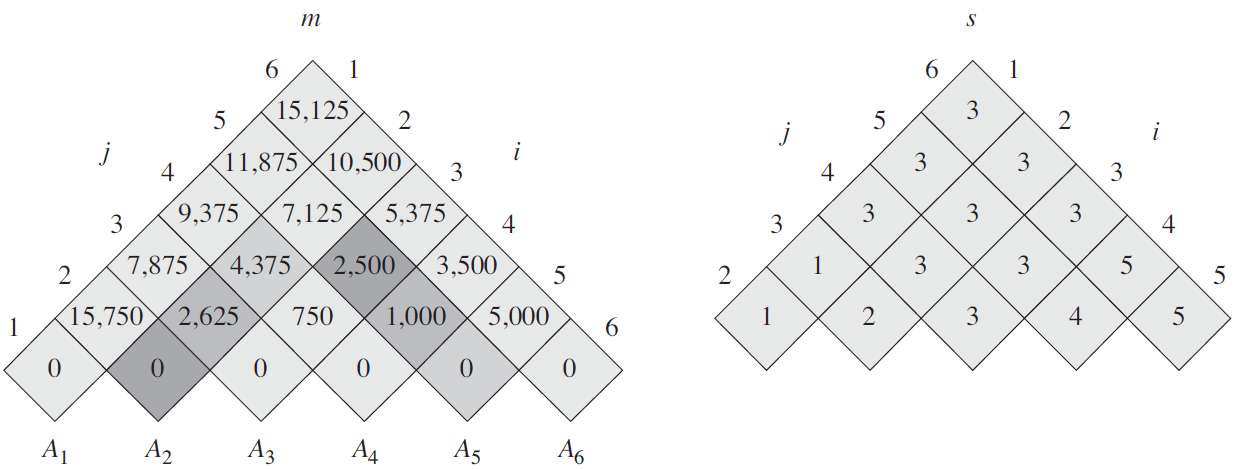
\includegraphics[width=\textwidth]{parenthesization}
    
    

    \item Construct an optimal solution from computed information.
\end{enumerate}
\end{document}